\documentclass[a4paper]{article}

\usepackage[english]{babel}
\usepackage[utf8]{inputenc}
\usepackage{hyperref}
\usepackage{amsmath}
\usepackage{float}
\usepackage[margin=0.5in]{geometry}
\usepackage{graphicx}
\usepackage[colorinlistoftodos]{todonotes}
\usepackage{subfig}
\usepackage{booktabs}


\title{10701 Project Interim Report \\
\Large{American Epilepsy Society Seizure Prediction Challenge}}

\author{Revanth Bhattaram (rbhattar) \\ 
Archit Karandikar (akarandi) \\ 
Vipul Singh (vipuls)}

\date{\today}

\begin{document}
\maketitle

\section{Question and Goals}

\subsection{The Problem} 
Seizure forecasting systems have the potential to help patients with epilepsy lead more normal lives. Our project is based on a \href{https://www.kaggle.com/c/seizure-prediction}{kaggle} competition wherein the task is to distinguish between ten minute long data clips covering an hour prior to a seizure, and ten minute iEEG clips of interictal activity. The goal of the competition is to demonstrate the existence and accurate classification of the preictal brain state in dogs and humans with naturally occurring epilepsy.

\subsection{Metrics} 
Being a Kaggle contest, one well-defined metric for success is the score provided by the contest platform. For each clip in the test set, we predict a real-valued probability that a given clip is preictal. The score is computed based on the area under the \href{http://en.wikipedia.org/wiki/Receiver_operating_characteristic}{ROC} curve (AUC). \\

We have also developed a K-fold cross-validation framework which helps us judge performance via F-score. We want high recall on preictal segments, so we use weighted F-score. The rationale behind this is that for our use-case, it is important for us to not have false negatives (a patient should always be made aware before a seizure).

\subsection{Goals}
The minimum goal is to achieve good recall because that would mean that we are able to predict preictal states correctly and hence enable provision of relief to epilepsy-afflicted patients. We would specifically want to beat the bonehead model. \\
From the perspective of learning, we aim to apply various learning/classification algorithms suited to our problem, and study their pros and cons, and why some of them work well and others don't, based on our understanding of the data.

\section{Dataset}
Intracranial EEG was recorded from dogs with naturally occurring epilepsy using an ambulatory monitoring system. Datasets from patients with epilepsy undergoing intracranial EEG monitoring to identify a region of brain that can be resected to prevent future seizures are also included in the contest. These are available at \url{https://www.kaggle.com/c/seizure-prediction/data}. 
\begin{itemize}
\item \textbf{Training Data Set} : This is organized into one hour sequences of ten-minute iEEG clips labeled `Preictal' for pre-seizure data segments, or `Interictal' for non-seizure data segments. The interictal activity data, in the case of canines, is recorded at least a week before and after a seizure. For human training data, the interictal training data is recorded at least 4 hours before and after a seizure. The preictal activity data is recorded one hour prior to a seizure with a 5 minute offset.
\item \textbf{Test Data Set} : For each subject (5 dogs and 2 patients), it consists of 10 minute iEEG clips which are
provided in random order. 
\end{itemize}

\subsection{Preliminary Analysis}
\label{prelim}
The first step taken was to plot the EEG sample values for the various subjects/electrodes and see if we could derive information out of them. An example of such a plot is shown in Figure~\ref{fig:eeg}.

\begin{figure}
  \centering
    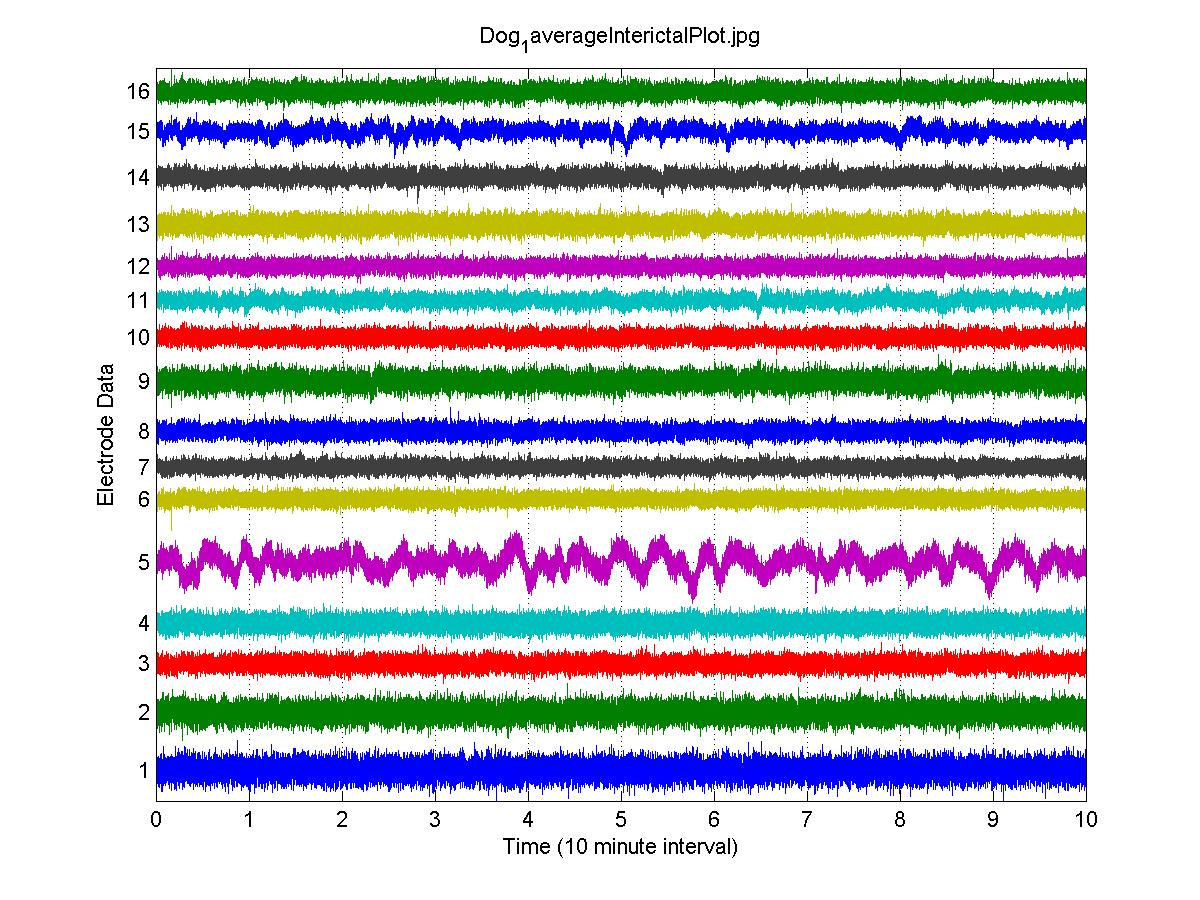
\includegraphics[width=0.8\textwidth]{EEGPlot.jpg}
  \caption{Plot of electrode-wise average EEG signal activity for a 10-minute segment. x-axis represents time in minutes}
  \label{fig:eeg}
\end{figure}

Plots for interictal and preictal data segments were made in an attempt to see if there were any major differences that we could spot. Although, we weren't able to derive too much information from these plots (other than the existence of outlier data segments), it did serve as a motivation to try Fourier methods (described later on).

\subsection{Extracting Basic Features}
We managed to calculate basic statistics like the mean/variance of each data segment over all subjects. This data is used to construct the feature vectors in our bonehead model.

The general trend that we observed was that the variance of the preictal data was lesser than that of the interictal data. This is illustrated in the following heatmap:

\begin{figure}[H]
    \centering
    \subfloat[interictal]{{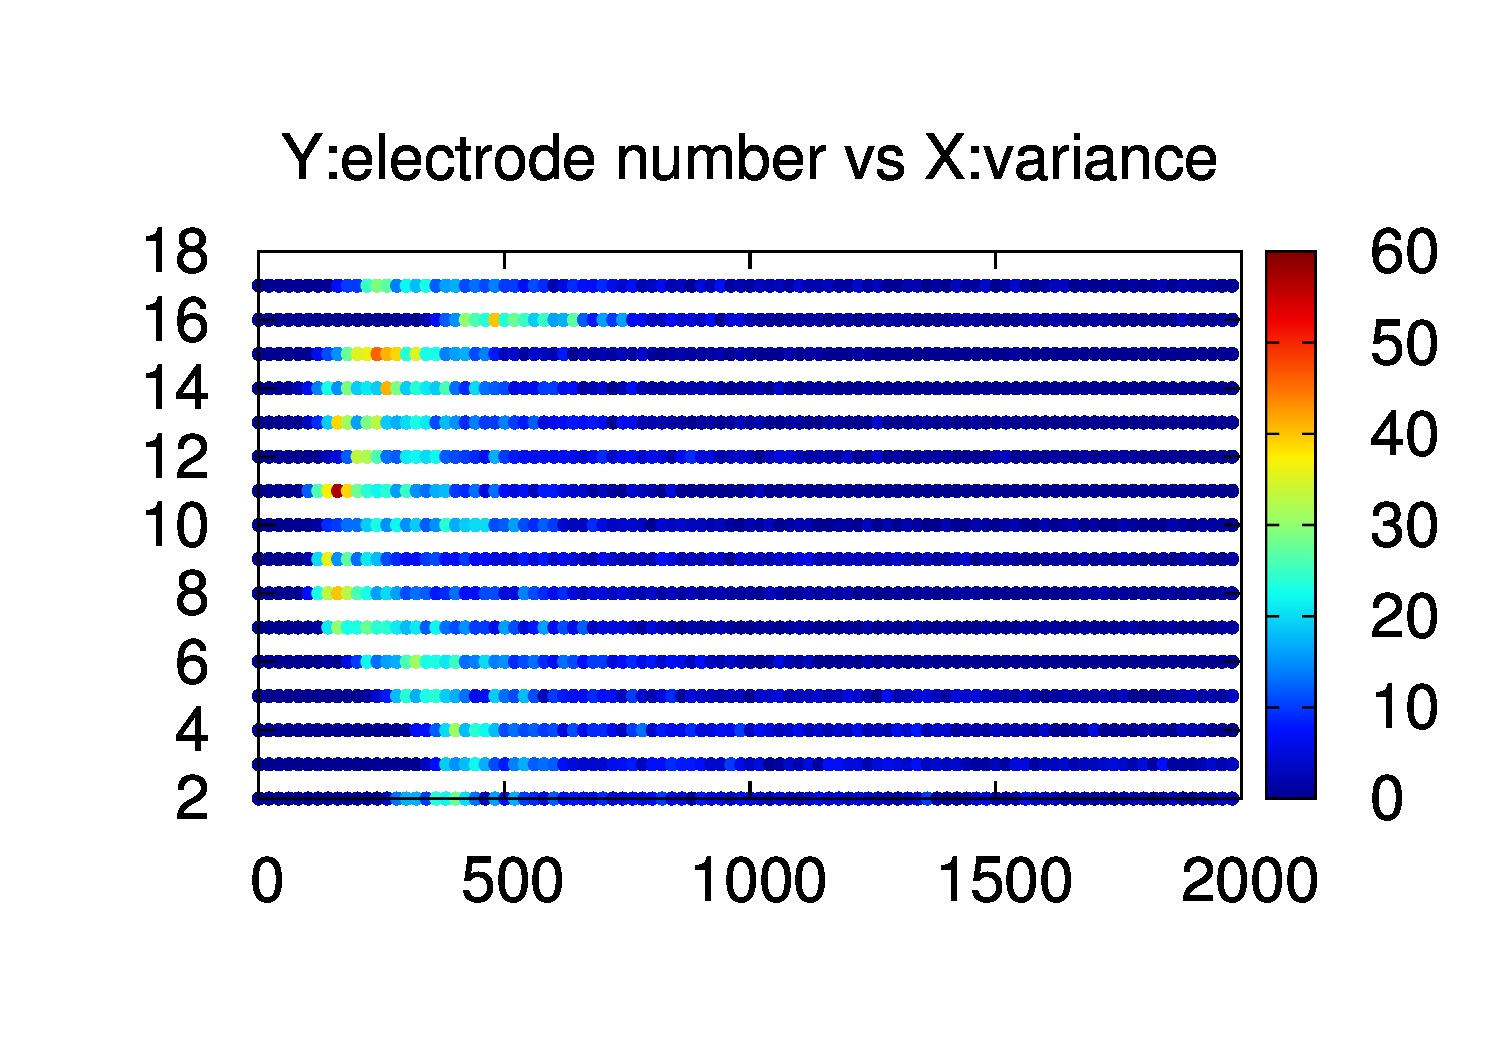
\includegraphics[width=0.4\linewidth]{Dog_2_interictal_heatmap.jpg} }}%
    \qquad
    \subfloat[prerictal]{{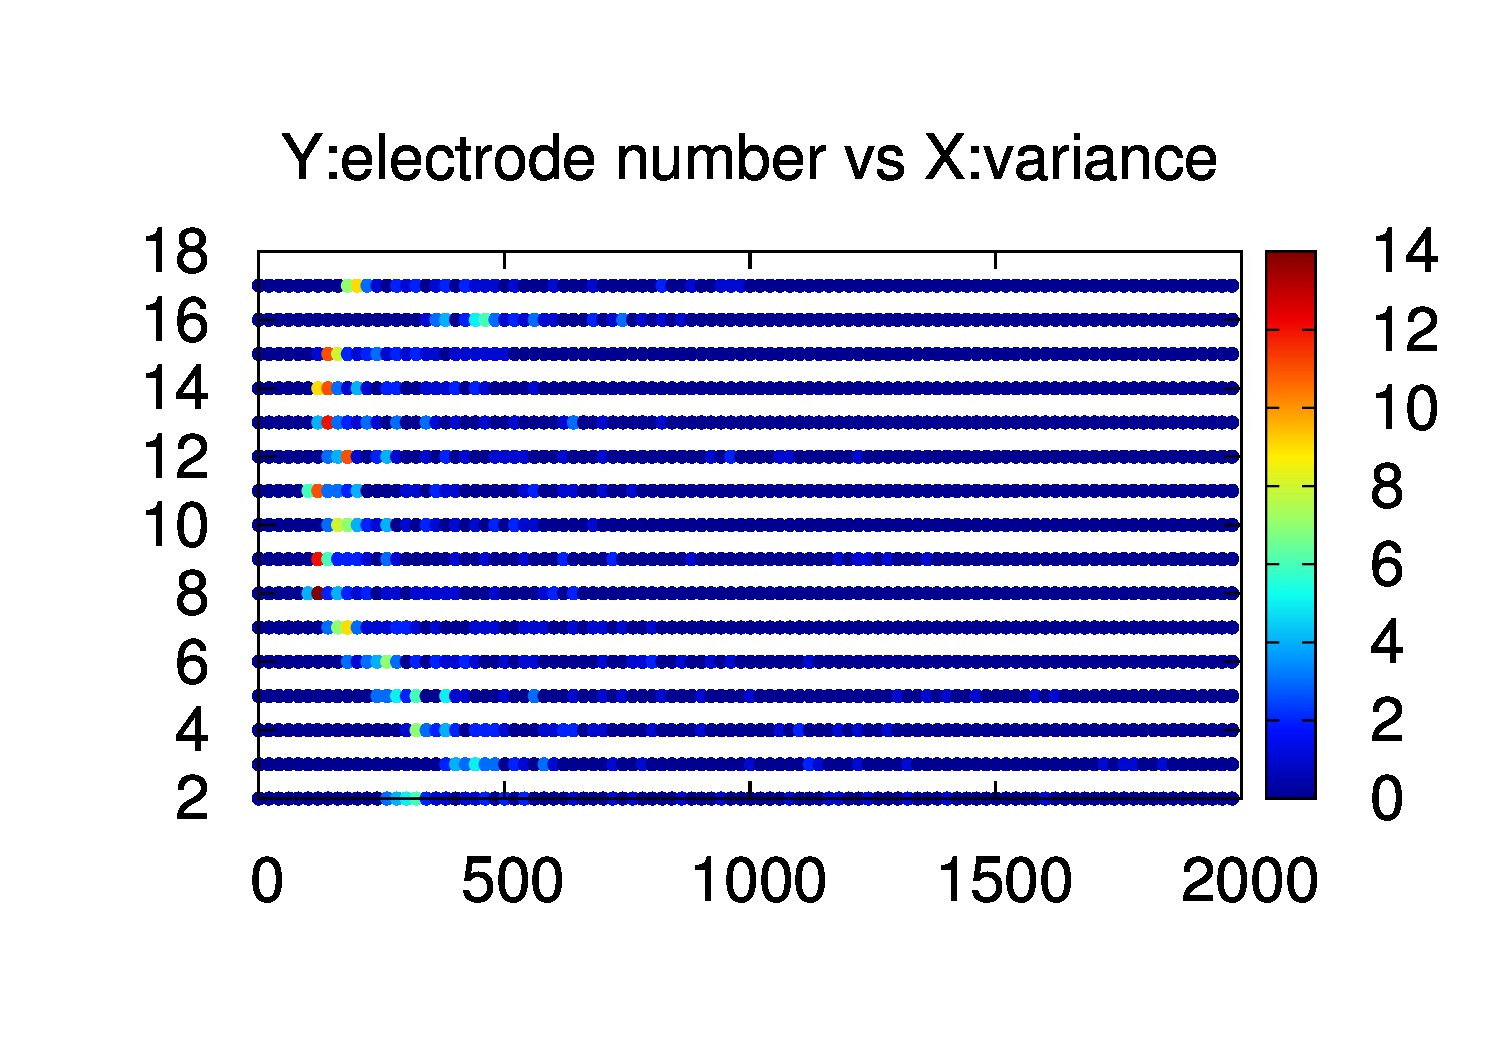
\includegraphics[width=0.4\linewidth]{Dog_2_preictal_heatmap.jpg} }}%
    \caption{Heat maps showing the distibution of variance for every electrode for Dog  2}%
    \label{fig:heatvar}%
\end{figure}

\subsubsection{Trying To Find A Correlation}

Another statistic that we managed to calculate was the covariance matrix of data segments. Following that, we calculated the correlation coefficient matrix for each data segment and tried to see if they would give us any information about correlation between electrodes. To observe this, we used heatmaps (Figure \ref{fig:corrMatrix}) for interictal data and preictal data.

\begin{figure}[H]
    \centering
    \subfloat[Interictal]{{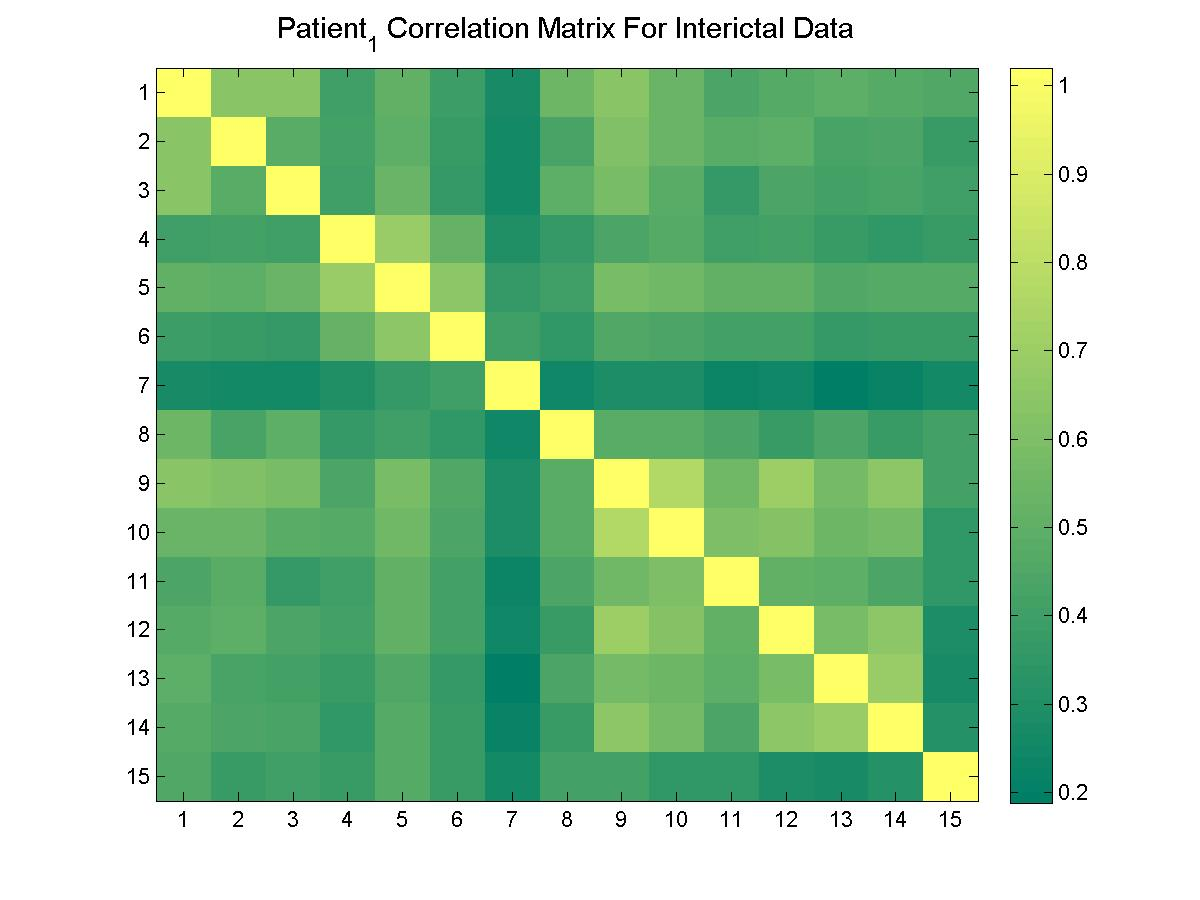
\includegraphics[width=0.4\linewidth]{InterictalCorrelation.jpg} }}%
    \qquad
    \subfloat[Preictal]{{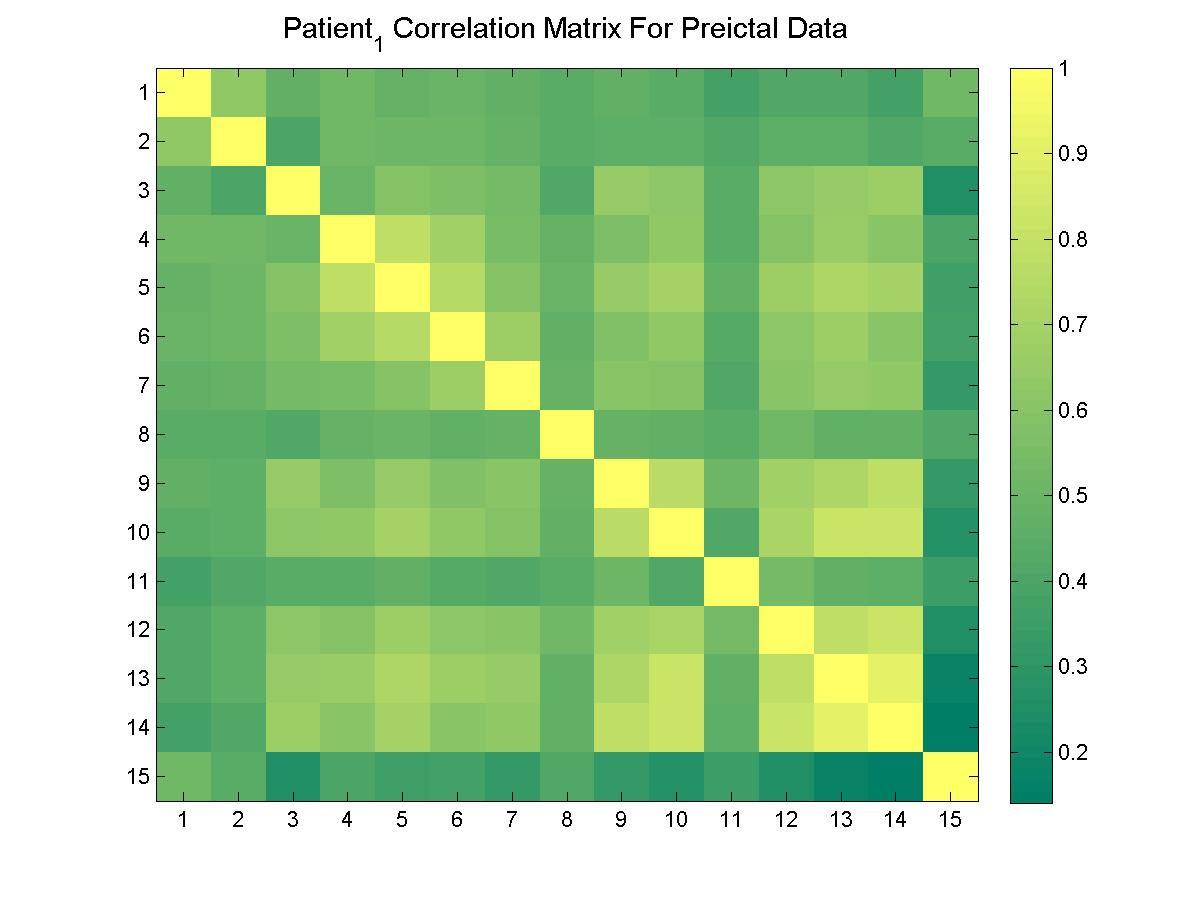
\includegraphics[width=0.4\linewidth]{PreictalCorrelation.jpg} }}%
    \caption{Correlation Coefficient Matrix for the two states}%
    \label{fig:corrMatrix}%
\end{figure}

In the heatmap plots, a box with a more intense color (according to the color scale) would correspond to a pair of electrodes that have a high correlation coefficient (which is why the boxes in the diagonal have the most intense colors). Observe how the plot changes when we move from interictal to preictal. It becomes 'brighter'.  This means that there is more correlation between pairs of electrodes in the preictal state when compared to the interictal state. This difference gives us motivation to look for bivariate features which will be able to distinguish between preictal and interictal states better than a normal univariate feature. This assumption is supported in a study that has been carried out in \cite{lecun}.

\section{Testing Framework}
For testing purposes, we're using a K-Fold cross-validation approach. For each subject, the M training segments of interictal data and N segments of preictal data are divided into partitions of size $\frac{M}{K}, \frac{N}{K}$ respectively. Thus, we will have K subsamples that contain equal number of interictal and preictal training segments. \\
One of the subsamples is chosen for validation purposes while the rest are used to train the classifier. This is repeated for all K subsamples and we note down the average metric score. For this project, we're setting K=3 so that we have a decent number of preictal data segments for testing. 

The basic metric that could be used for evaluation is the average number of classification errors (or error percentage) of the classifier.

For our project, an important point to consider is that it is crucial for us to be able to predict the occurrence of a seizure given a preictal data segment (so that the patient may make preparations). False negatives (classifying a preictal segment as interictal) should be penalized more when compared to false positives(classifying an interictal segment as preictal). Thus, it is important for us to have a higher recall than precision. For that purpose we will be using the f-Measure metric (with higher weight on recall) $ = \frac{3PR}{2P + R} $ as our evaluation metric.

For our evaluation, we define,

$$\text{Precision} = \frac{\text{Number of Accurate Preictal Predictions}}{\text{Number of Preictal Predictions}}$$

$$\text{Recall} = \frac{\text{Number of Accurate Preictal Predictions}}{\text{Number of Preictal Segments in the Test Set}}$$

$$\text{Error Percentage} = \frac{\text{Number of Misclassifications made} * 100}{\text{Number of Testing Data Segments}}$$

\section{Models}
We've tried a couple of models for classification using basic features. For these models, our experimental set up is as shown in Table \ref{tab:data}.

\begin{table}[!htbp]
\centering
\begin{tabular}{*4c}
\toprule
Subject & Interictal data : Preictal data & $\#$ Training data & $\#$ Testing data\\
\midrule
Dog 1 & 480 : 24 & 336 & 168\\
Dog 2 & 500 : 42 & 361 & 181\\
Dog 3 & 1440 : 72 & 1008 & 504\\
Dog 4 & 804 : 97 & 601 & 300\\
Dog 5 & 450 : 30 & 320 & 160\\
Patient 1 & 50 : 18 & 45 & 23\\
Patient 2 & 42 : 18 & 40 & 20\\
\bottomrule
\end{tabular}
\caption{Data Used By The Models, during cross-validation}
\label{tab:data}
\end{table}

In Table \ref{tab:data}, the second column refers to the number of Interictal data segments we have vs the number of preictal data segments. Columns 3 \& 4 refer to the number of training and testing segments we will be using for our 3 fold cross validation framework.

It has to be noted that we will be building subject specific models (in terms of parameters). The underlying algorithm and feature extraction would remain same but while predicting for a given subject, we will only consider the relevant training data. We do not intend on building a `one size fits all' classifier. The merits of using patient specific classifiers have been studied in \cite{yunpark}.

\subsection{Bonehead Model}
For this model, we are considering the mean sample values for each electrode as the set of features for a data segment. For example, given a data segment of a subject with M electrodes, we would represent it with a 1 x M vector with each value representing the average data value for each electrode. \\
These data points are then fed to a Naive Bayes learner which generates a Gaussian Naive Bayes classifier.

The results of this classifier can be seen in Table \ref{tab:bonehead}.


\begin{table}[!htbp]
\centering
\resizebox{\linewidth}{!}{%
\begin{tabular}{c c c c c c c c c c c c c c}
\toprule
Subject & \multicolumn{4}{c}{Test on Fold 1} & \multicolumn{4}{c}{Test on Fold 2} & \multicolumn{4}{c}{Test on Fold 3} & MeanError\\
\midrule
 & Errors  & Precision & Recall  & f-Measure  &  Errors  & Precision & Recall & f-Measure	& Errors  & Precision & Recall & f-Measure\\
Dog 1 &  7.74\% & 0.27 & 0.38 & 0.33 &  12.5\% & 0.16 & 0.38 & 0.26 &  10.12\% & 0.15 & 0.25 & 0.21 & 10.12\%\\
Dog 2 &  10.5\% & 0.42 & 1.0 & 0.69 &  15.47\% & 0.28 & 0.64 & 0.45 &  9.39\% & 0.45 & 1.0 & 0.71 & 11.78\%\\
Dog 3 &  5.75\% & 0.0 & 0.0 & 0 &  4.56\% & 1.0 & 0.04 & 0.06 &  5.95\% & 0.0 & 0.0 & 0 & 5.42\%\\
Dog 4 &  10.33\% & 1.0 & 0.03 & 0.05 &  11.0\% & 0.0 & 0.0 & 0 &  11.33\% & 0.0 & 0.0 & 0 & 10.89\%\\
Dog 5 &  8.75\% & 0.36 & 0.5 & 0.44 &  8.13\% & 0.33 & 0.3 & 0.31 &  16.88\% & 0.16 & 0.4 & 0.27 & 11.25\%\\
Patient 1 &  34.78\% & 0.25 & 0.17 & 0.19 &  26.09\% & 0.0 & 0.0 & 0 &  21.74\% & 0.67 & 0.33 & 0.4 & 27.52\%\\
Patient 2 &  30.0\% & 0.5 & 0.17 & 0.21 &  50.0\% & 0.17 & 0.17 & 0.17 &  35.0\% & 0.0 & 0.0 & 0 & 38.35\%\\
\bottomrule
\end{tabular}
}
\caption{Performance of the bonehead model.}
\label{tab:bonehead}
\end{table}

Running this classifier on the testing data for the Kaggle competition yielded a score of 0.54067.

\subsection{More Features and a Different Learner}
As a second approach, we decided to use the variances of each electrode and correlation coefficients between each pair of electrodes as a feature vector for each data segment. So, for a subject with M electrodes, we'd represent each data segment with a vector of size M (variance of each electrode) + $\frac{M(M-1)}{2}$ (correlation coefficients between all pairs). \\
We then feed these data points to a regression tree learner which generates a classifier for us.

We obtained better results (Table \ref{tab:regtree}) when compared to the bonehead model.

\begin{table}[!htbp]
\centering
\resizebox{\linewidth}{!}{%
\begin{tabular}{c c c c c c c c c c c c c c}
\toprule
Subject & \multicolumn{4}{c}{Test on Fold 1} & \multicolumn{4}{c}{Test on Fold 2} & \multicolumn{4}{c}{Test on Fold 3} & MeanError\\
\midrule
 & Errors  & Precision & Recall  & f-Measure  &  Errors  & Precision & Recall & f-Measure	& Errors  & Precision & Recall & f-Measure\\
Dog 1 &  11.9\% & 0.13 & 0.25 & 0.19 &  6.55\% & 0.2 & 0.13 & 0.14 &  5.95\% & 0.25 & 0.13 & 0.15 & 8.14\%\\
Dog 2 &  6.08\% & 0.59 & 0.71 & 0.67 &  9.94\% & 0.33 & 0.29 & 0.3 &  4.97\% & 0.69 & 0.64 & 0.66 & 7.0\%\\
Dog 3 &  6.75\% & 0.31 & 0.33 & 0.32 &  6.35\% & 0.33 & 0.33 & 0.33 &  6.55\% & 0.32 & 0.33 & 0.33 & 6.55\%\\
Dog 4 &  14.33\% & 0.32 & 0.28 & 0.29 &  15.0\% & 0.32 & 0.37 & 0.35 &  12.33\% & 0.42 & 0.4 & 0.41 & 13.89\%\\
Dog 5 &  7.5\% & 0.43 & 0.6 & 0.53 &  4.38\% & 0.64 & 0.7 & 0.68 &  6.25\% & 0.5 & 0.6 & 0.56 & 6.04\%\\
Patient 1 &  21.74\% & 0.56 & 0.83 & 0.71 &  26.09\% & 0.5 & 0.33 & 0.38 &  21.74\% & 0.55 & 1.0 & 0.78 & 23.17\%\\
Patient 2 &  25.0\% & 0.6 & 0.5 & 0.53 &  45.0\% & 0.0 & 0.0 & 0 &  45.0\% & 0.29 & 0.33 & 0.32 & 38.35\%\\

\bottomrule
\end{tabular}
}
\caption{Performance of the regression tree model.}
\label{tab:regtree}
\end{table}

Running this classifier on the testing data for the Kaggle competition yielded a score of 0.57031.

\subsection{7-Class classification}
The training data is labeled with sequence numbers which identify the 10-minute interval within an hour. One of the approaches that we tried was separating the preictal class into 6 classes corresponding to the 6 sequence types. The rationale underlying this model was that one would expect the ``preictalness" of a preictal segment to increase markedly with time in the hour before the seizure unlike the ``interictalness" of an interictal segment. We conducted several analyses of the test data in an attempt to find evidence to support this intuition. Figure \ref{fig:meanvar} demonstrates the results of two of our experiments:

\begin{figure}[H]
    \centering
    \subfloat[Mean]{{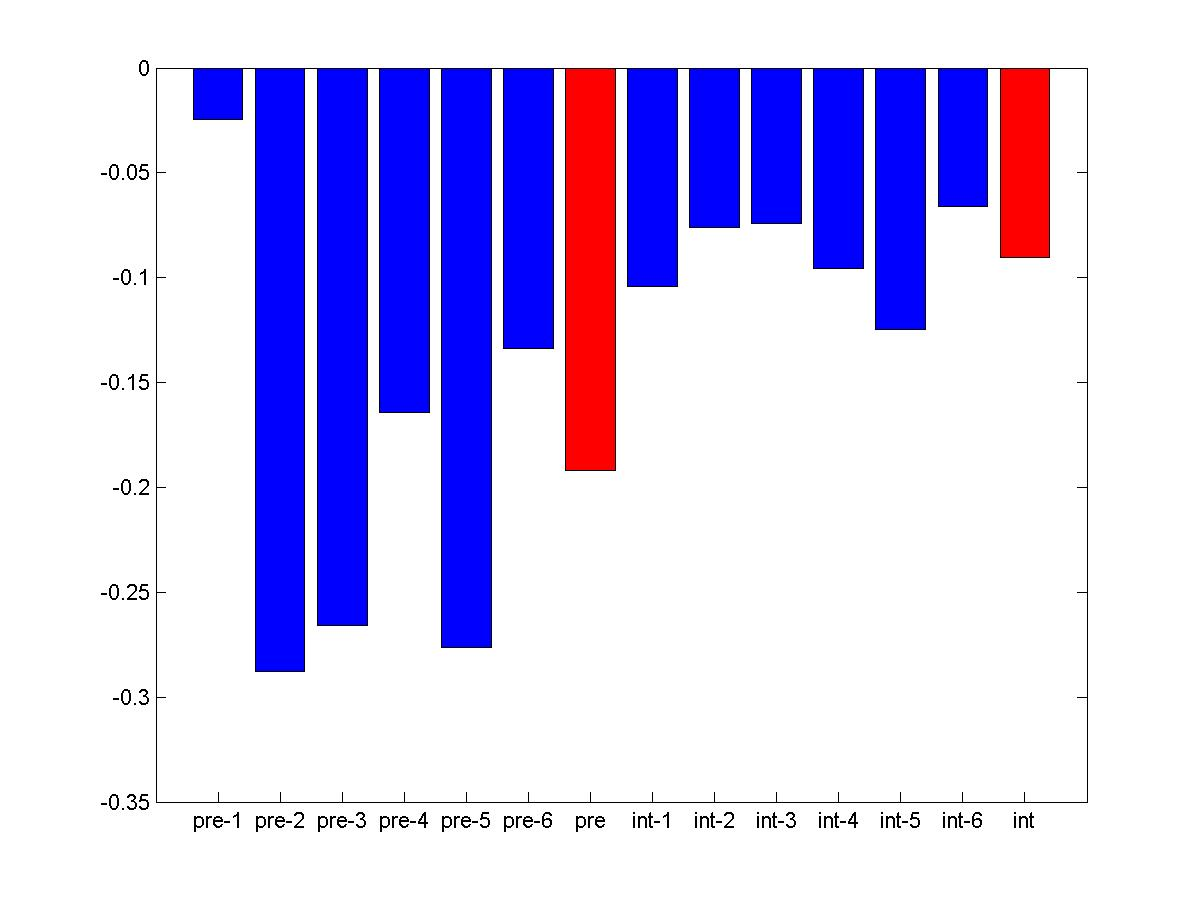
\includegraphics[width=0.4\linewidth]{Dog_2_Electrode_4_mean.jpg} }}%
    \qquad
    \subfloat[Variance]{{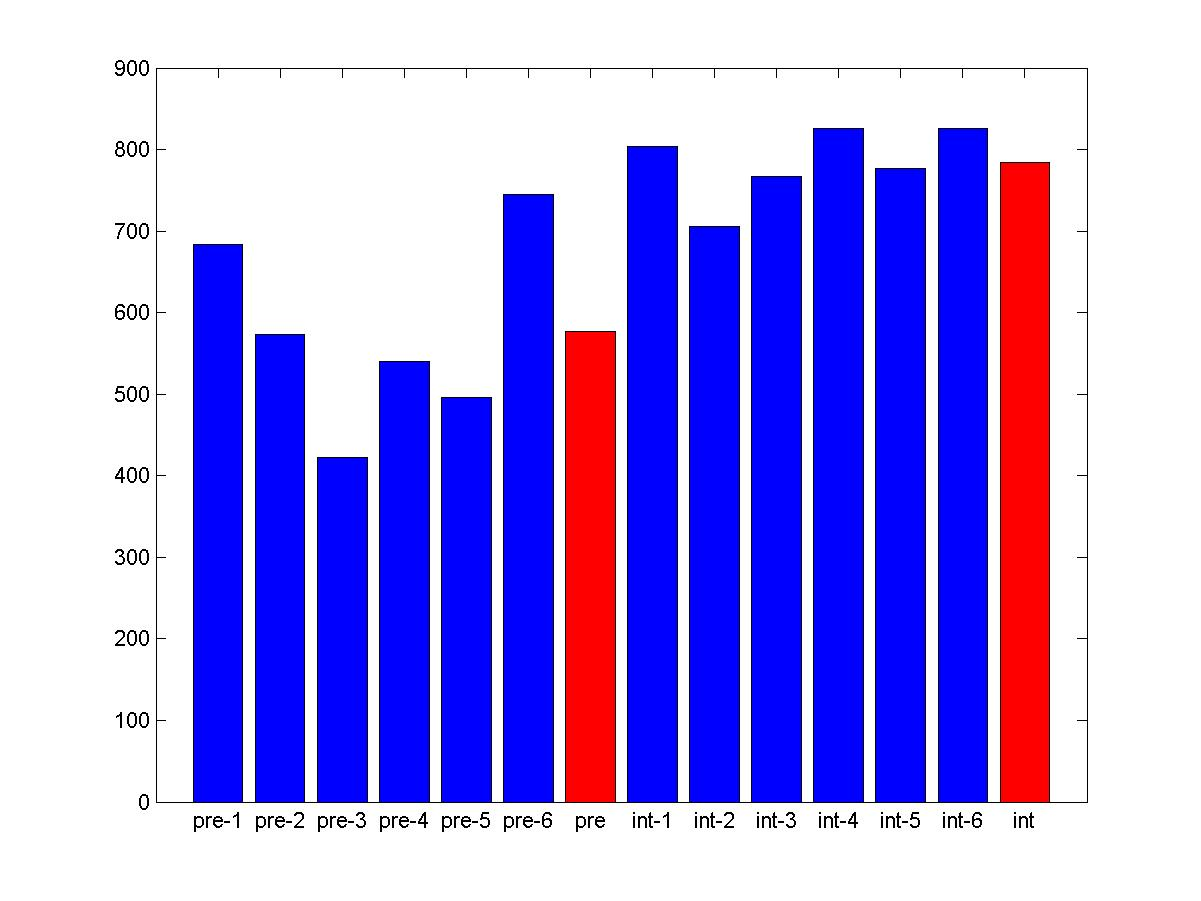
\includegraphics[width=0.4\linewidth]{Dog_2_Electrode_4_var.jpg} }}%
    \caption{Segment-specific (averaged) mean and variance for Dog 2 and Electrode 4}%
    \label{fig:meanvar}%
\end{figure}

This analysis showed us the general trend of interictal variances being higher than preictal variances. We also observed that in general, the 6 interictal means for a given subject-electrode pair were clustered together as compared to the preictal means. However we did not observe any clear trend across all subjects which could help us differentiate between the 6 preictal classes.

In contrast, the Fourier analysis presented in the following section showed clear patterns which could be used to differentiate between preictal and interictal data. Hence, we plan to focus on binary classification with Fourier Analysis in the future although we have not completely ruled out the 7-class classification model.

\section{Fourier Analysis}
As observed from the EEG graphs in \ref{prelim}, the signals from each electrode in a segment are quite periodic. Hence, we can apply Fourier Analysis on these signals to obtain amplitude spectrum over a range of frequencies. Below, we summarize our experiments relating to this: 

\subsection{Principal Frequencies}
We calculated the principal frequencies, i.e., the ones with maximum amplitude in the Fourier spectrum, for each electrode in each segment. Then, we took mean over all electrode-wise principal frequencies for a subject, and were able to get good separation between preictal and interictal segments. As an example, for Dog\_1, we obtain the following mean principal frequencies for the 16 electrodes:
\begin{verbatim}
Interictal: 3867.78, 4096.75, 3599.67, 3868.21, 2939.63, 4004.51,  3466.96, 3626.42, 3909.99, 3570.29,
2132.14, 3714.86, 3547.74, 3577.10, 3260.36, 3636
Preictal: 518.46, 294.71, 504.17, 756.04, 559.5, 1320.29, 277.58,  868.46, 1200.33, 449.88, 968.17, 
754.33, 647.71, 1141.58, 752.25, 487.38
\end{verbatim} 
On taking a closer look at the individual principal frequencies, we observe that there are some huge outliers, in the range of $10^{5}$ to $10^{6}$, while the smaller values are all clustered in ranges of around 0-200 Hz, for both preictal as well as interictal segments. 

\subsection{Outlier Detection}
To deal with the above-mentioned issue of outliers, we filtered the electrode-wise principal frequencies and retained only those segments where the frequencies were less than 10 times the average values for their respective electrodes. On doing so, we observed that the principal frequencies for both interictal as well as preictal data had clustered in the range 0-100 Hz. This is depicted via the sample heatmaps in figure \ref{d1freq}. Hence, just the set of principal frequencies doesn't seem to be a good distinguishing feature. We have, in a way, aggregated a 10-minute signal into one value, which leads to loss of information.

\begin{figure}[H]
	\centering
	\subfloat[Interictal]
{{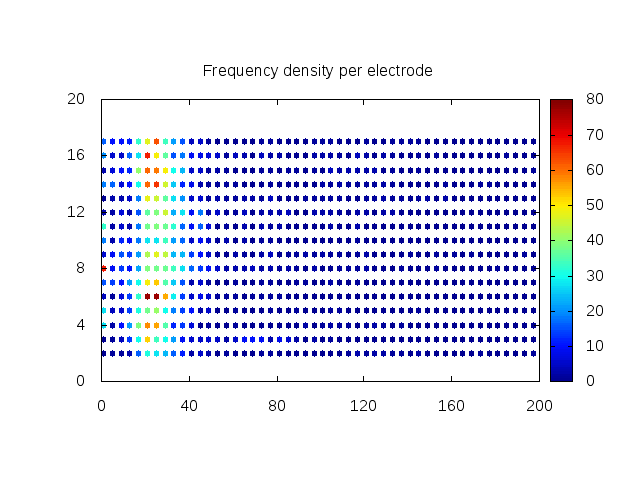
\includegraphics[width=0.4\linewidth]
{d1i.png} }}
	\qquad
	\subfloat[Preictal]
{{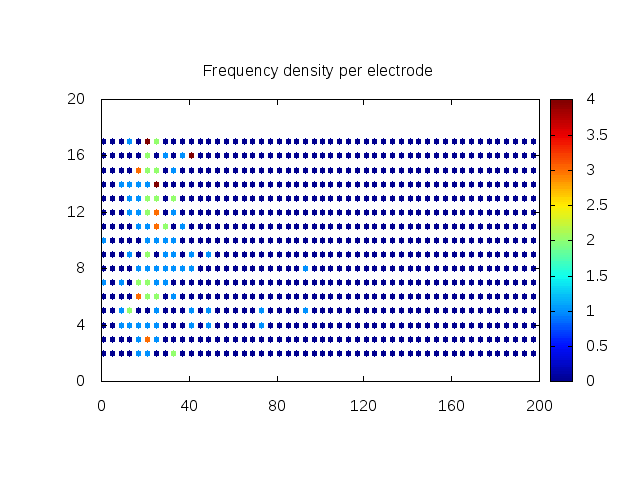
\includegraphics[width=0.4\linewidth]
{d1p.png} }}
	\caption{Heatmaps showing distribution of electrode-wise principal frequency for Dog1 data. x-axis represents frequency in Hertz.}
	\label{d1freq}
\end{figure}

\subsection{Fourier Spectra}
\label{spec}
Next we looked at the spectrum of amplitudes obtained from a Fourier decomposition on each electrode's signals. Here, we observe marked differences among preictal and interictal spectra for some particular electrodes. A few representative examples can be seen in figures \ref{d1e5spec} and \ref{d2e10spec}. For both cases shown here, the interictal plots are more peaked towards frequencies close to 0. Thus, we can use the vector of amplitudes across a range of frequencies, say 0-200 Hz as a feature for distinguishing between pre- and inter-ictal segments. 

\begin{figure}[H]
	\centering
	\subfloat[Interictal]
{{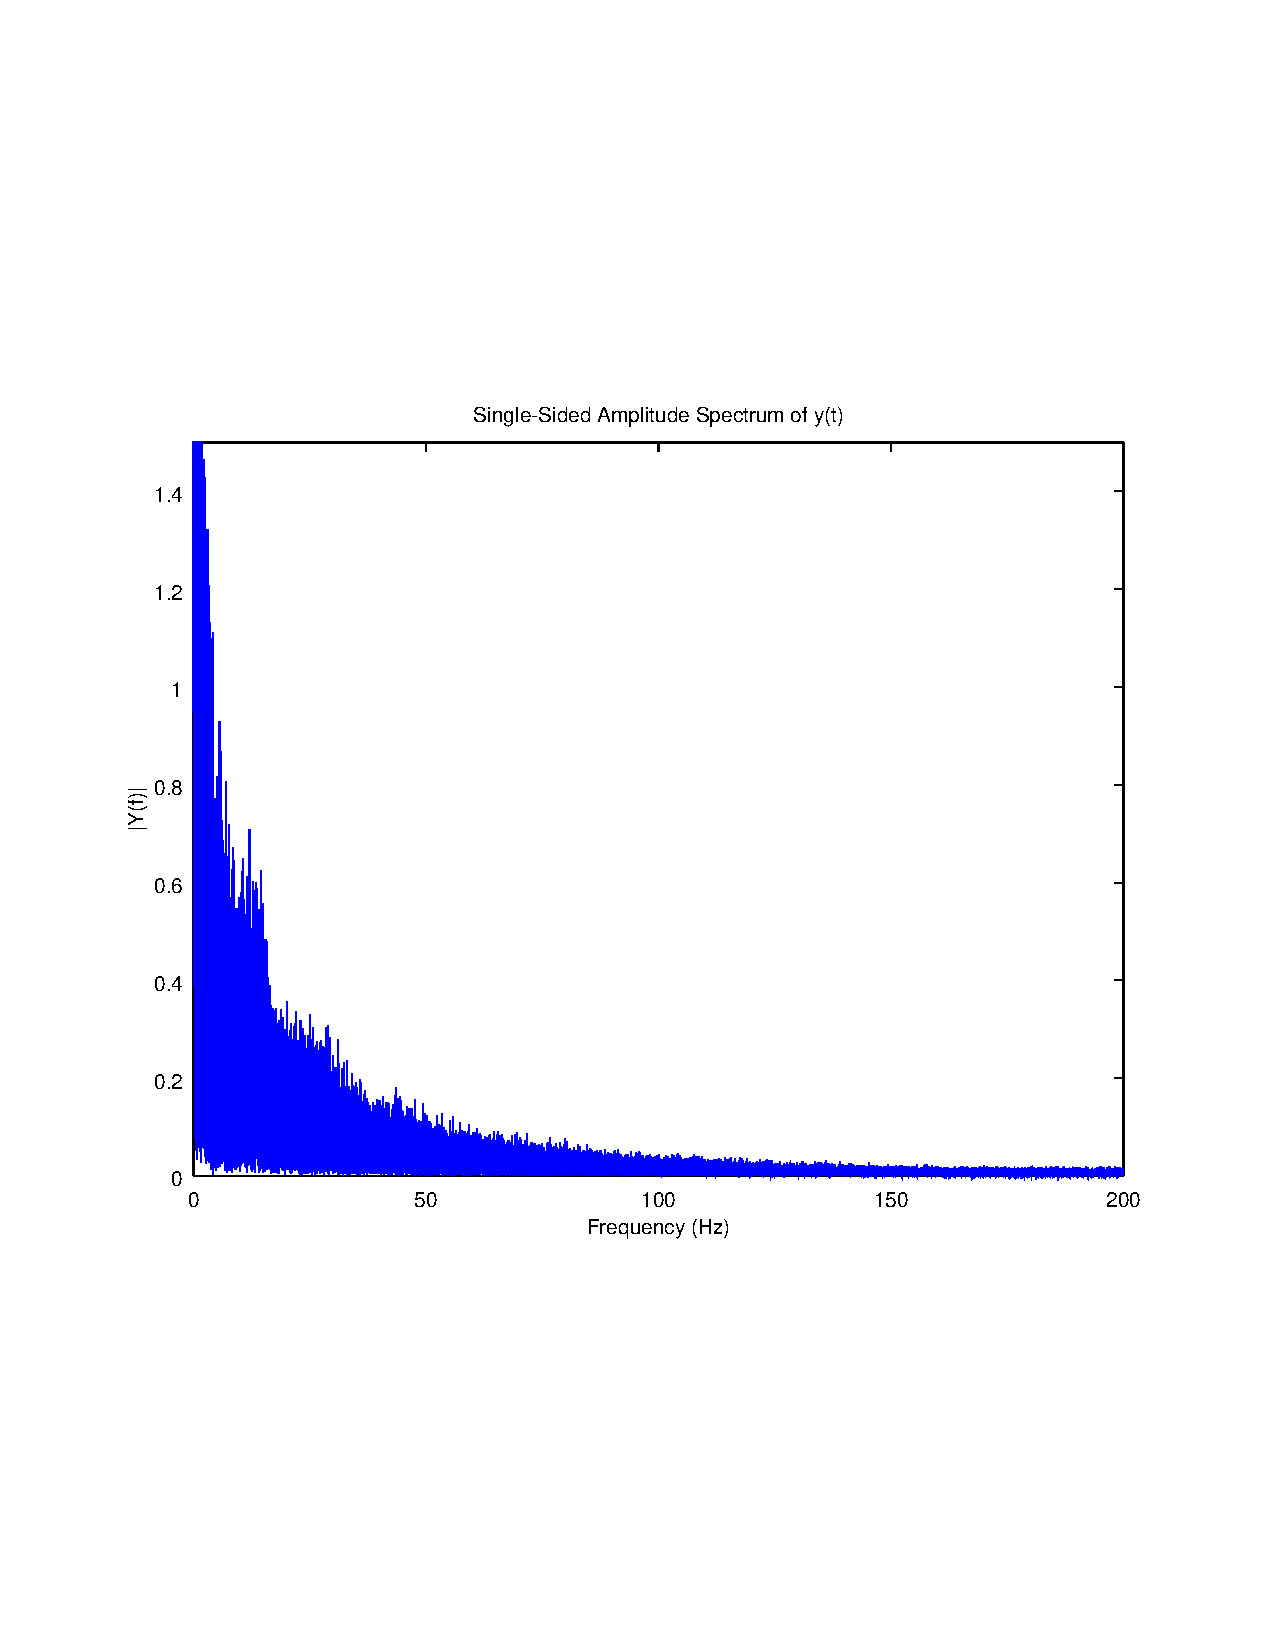
\includegraphics[width=0.4\linewidth]
{d1e5i11.pdf} }}
	\qquad
	\subfloat[Preictal]
{{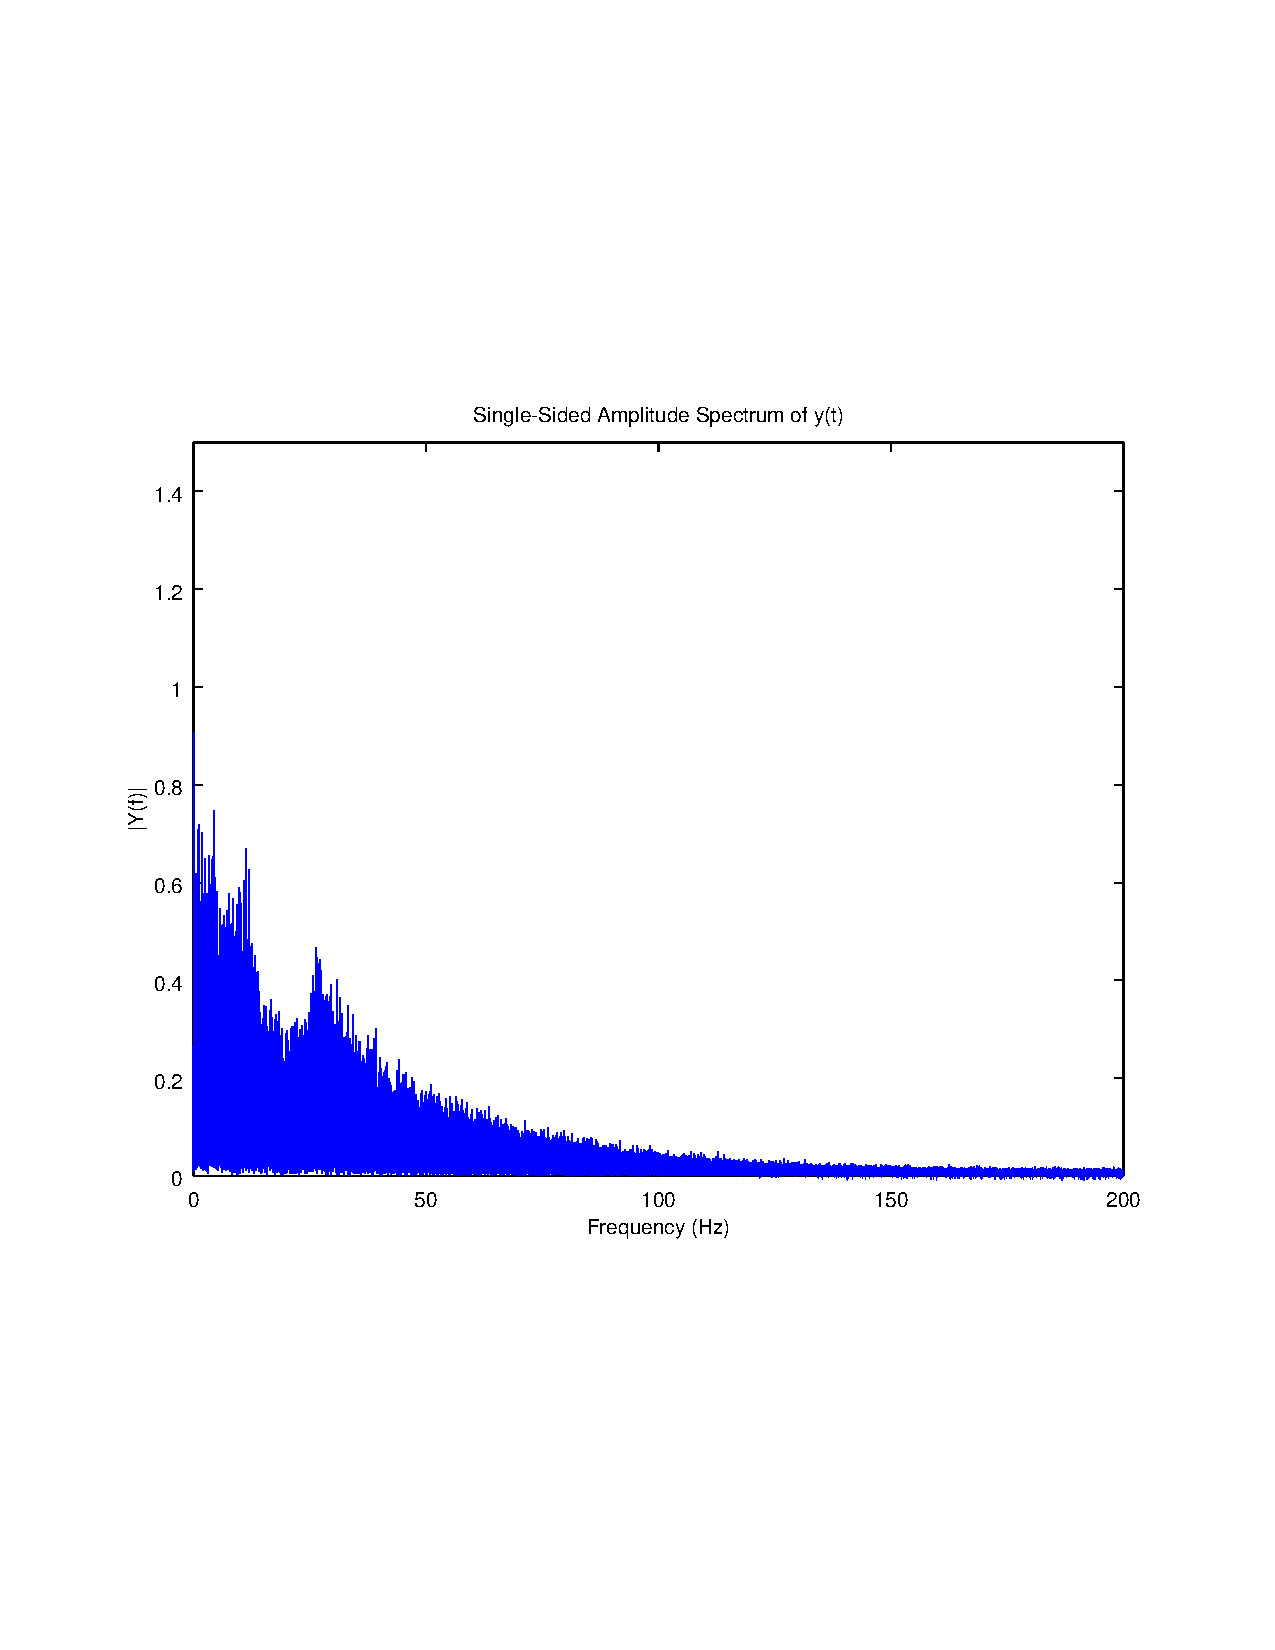
\includegraphics[width=0.4\linewidth]
{d1e5p23.pdf} }}
	\caption{Fourier spectra for the $5^{th}$ electrode in Dog1 data.}
	\label{d1e5spec}
\end{figure}

\begin{figure}[H]
	\centering
	\subfloat[Interictal]
{{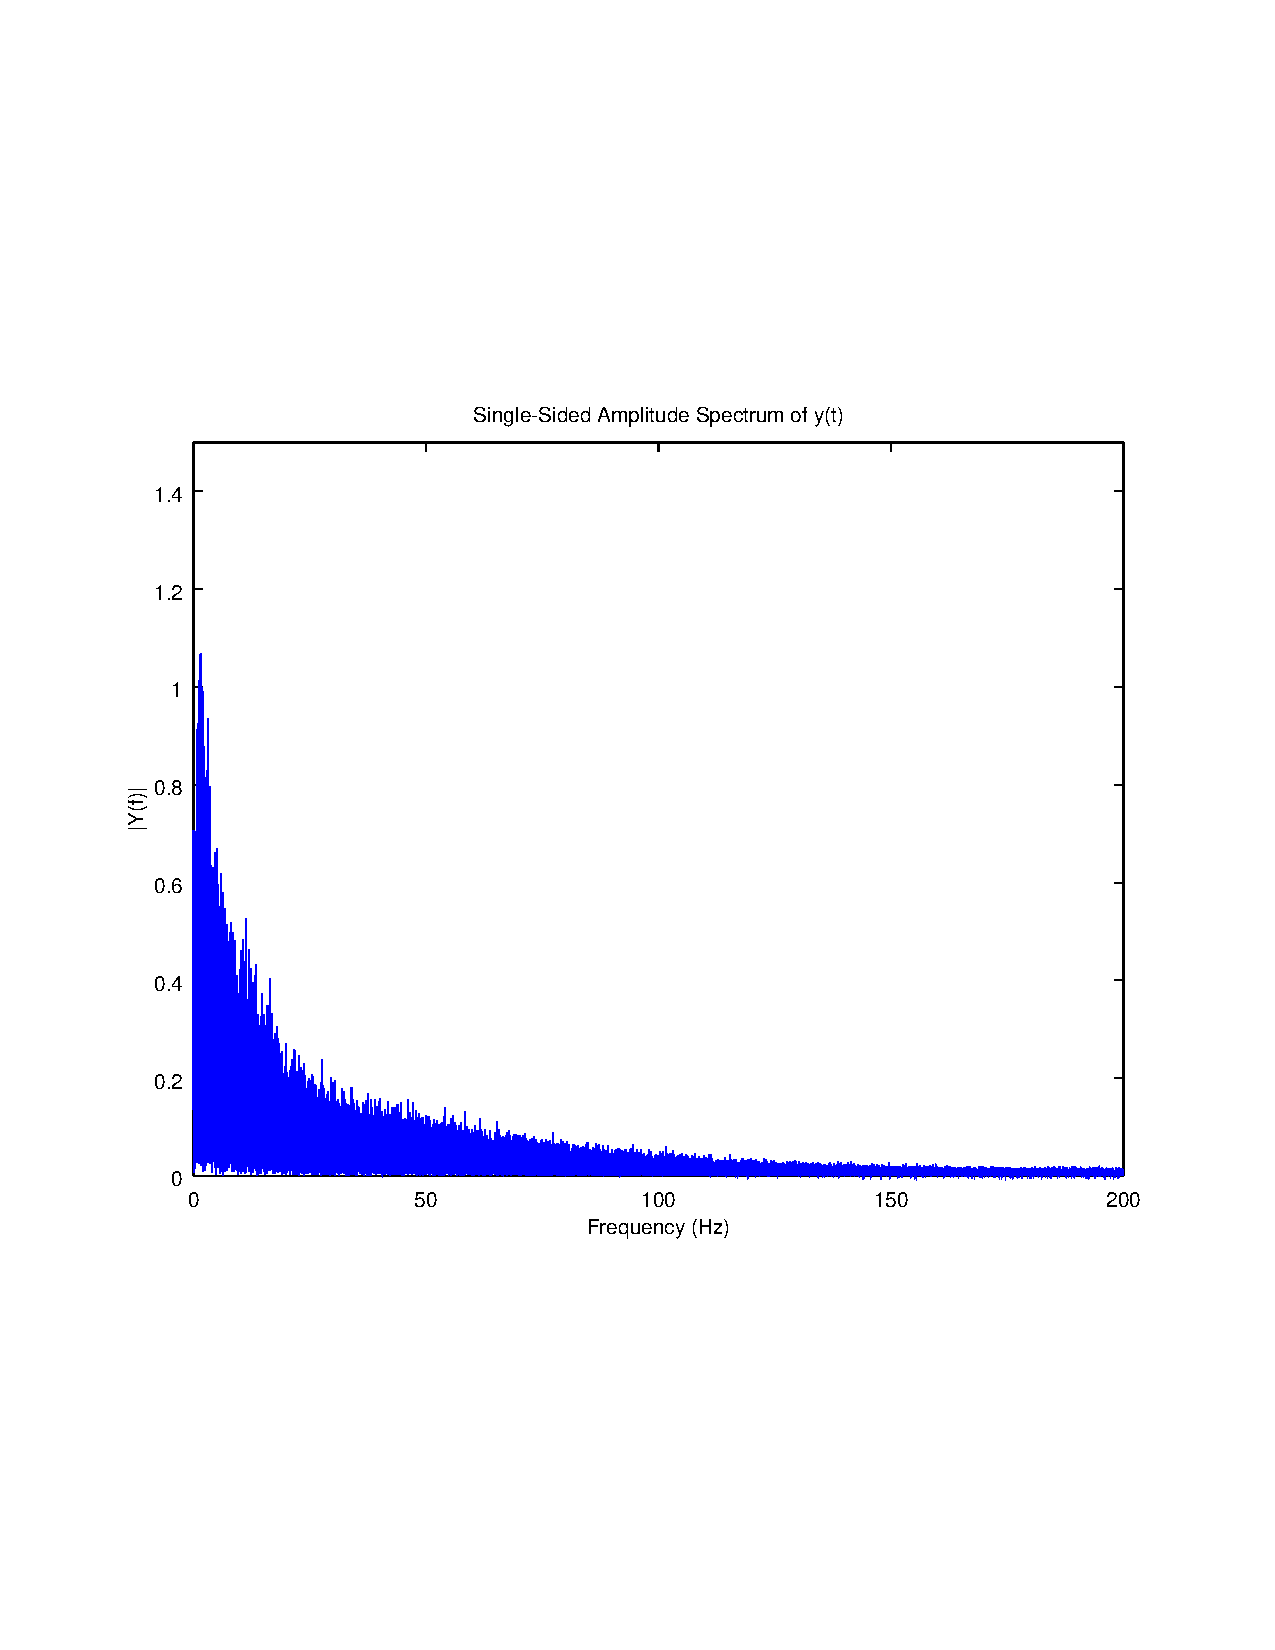
\includegraphics[width=0.4\linewidth]
{d2e10i1.pdf} }}
	\qquad
	\subfloat[Preictal]
{{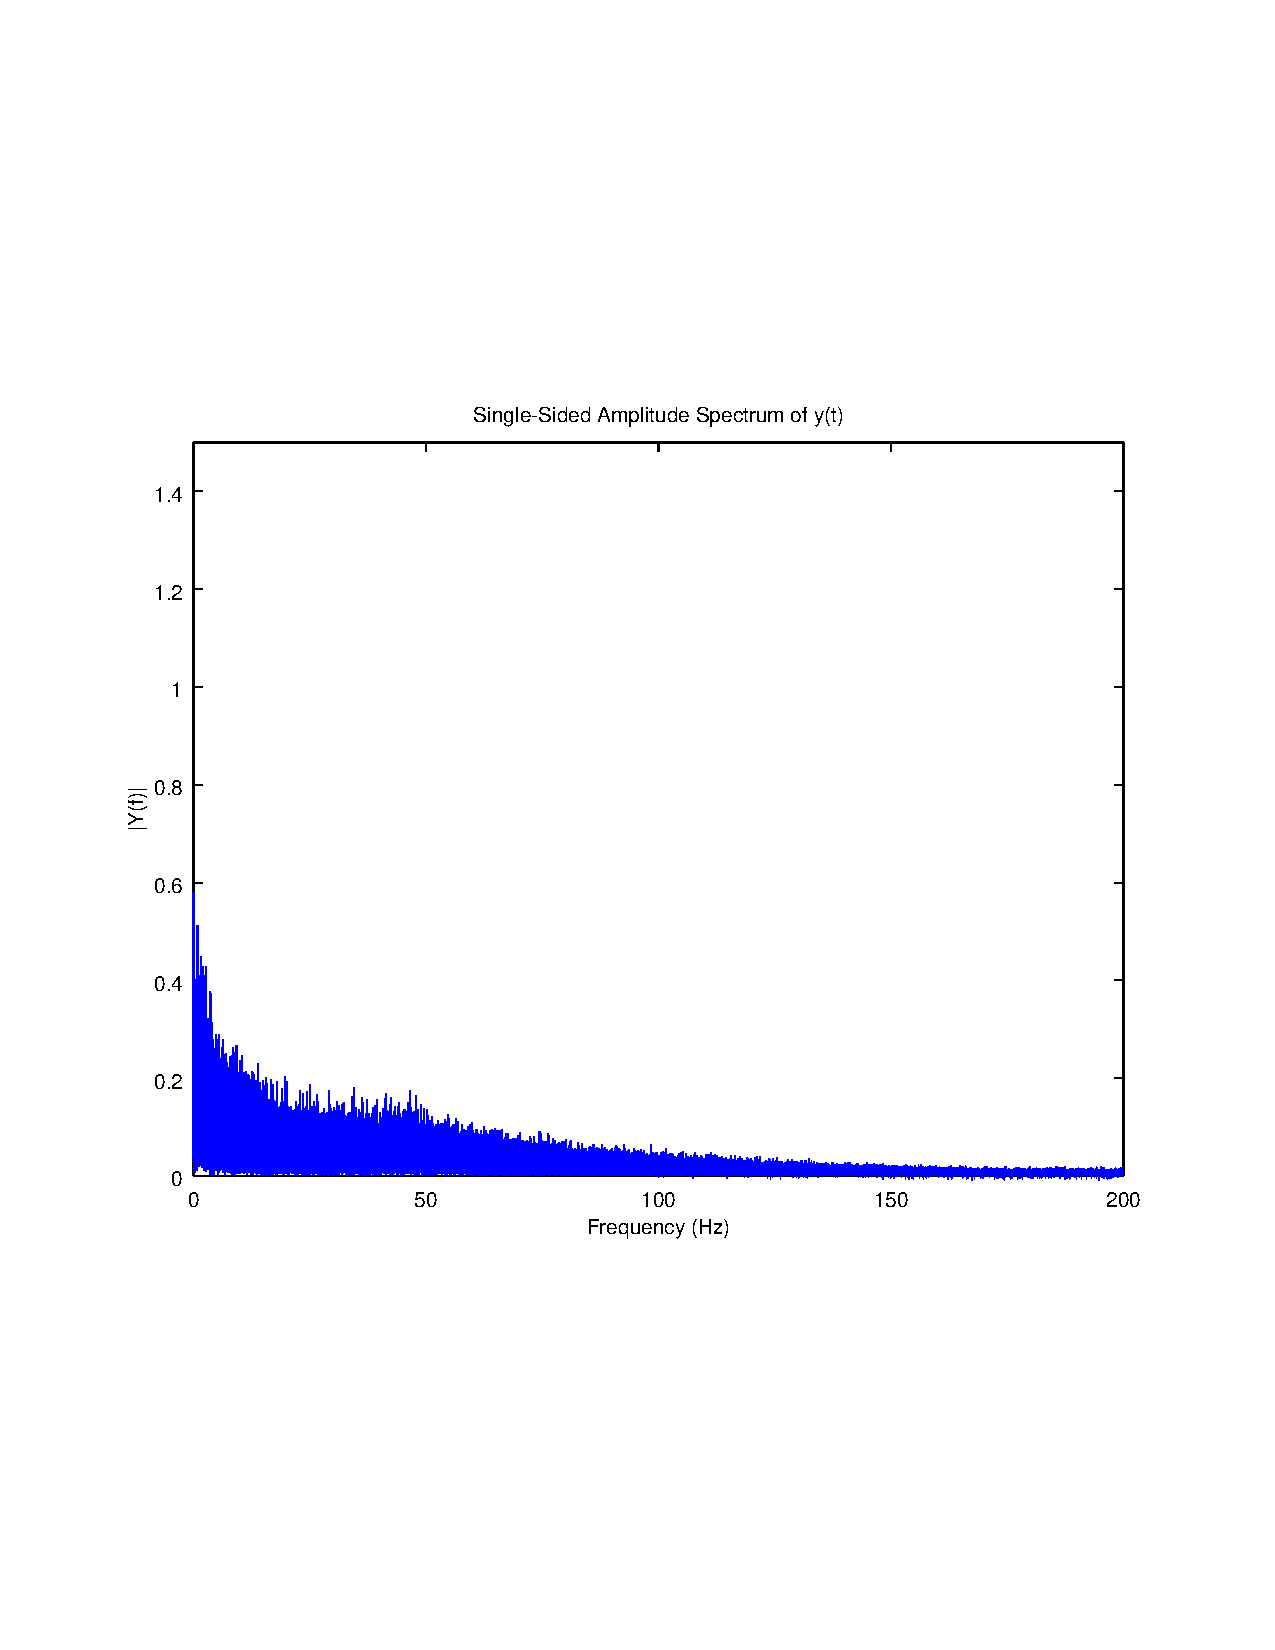
\includegraphics[width=0.4\linewidth]
{d2e10p1.pdf} }}
	\caption{Fourier spectra for the $10^{th}$ electrode in Dog2 data.}
	\label{d2e10spec}
\end{figure}

\section{Future Plan}
\subsection{Using bivariate features}
After filtering outliers, we plotted correlation heatmaps among electrode-pairs, looking at their principal frequencies, and obtained good distinction between the two classes of data. We therefore, plan to use such correlation matrices as bivariate features for our models, which is also supported in \cite{lecun}. In figure \ref{d1freqcorr}, we can see that there is more correlation among the electrodes in preictal segments, which is to be expected during a seizure.

\begin{figure}[H]
	\centering
	\subfloat[Interictal]
{{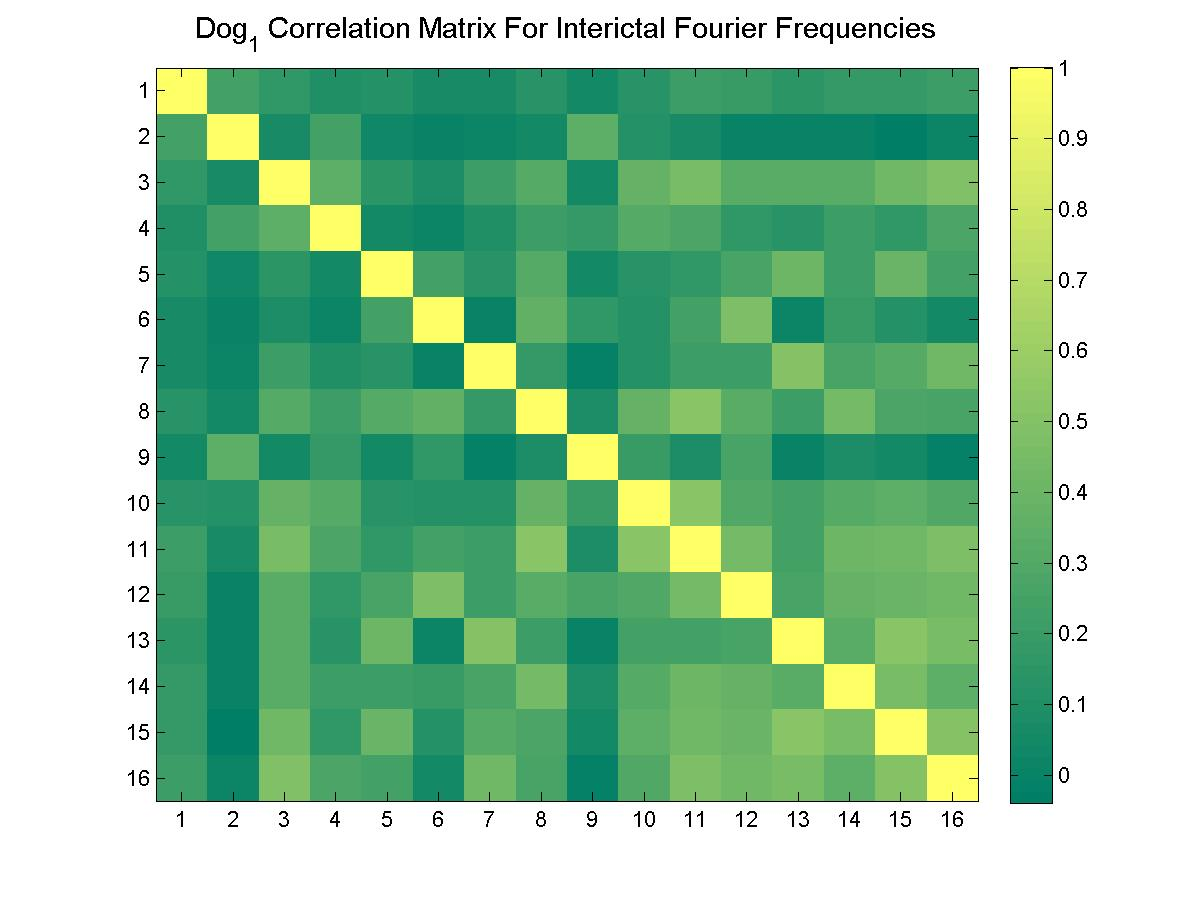
\includegraphics[width=0.4\linewidth]
{Dog1_InterictalFourierCorrelationPlot.jpg} }}
	\qquad
	\subfloat[Preictal]
{{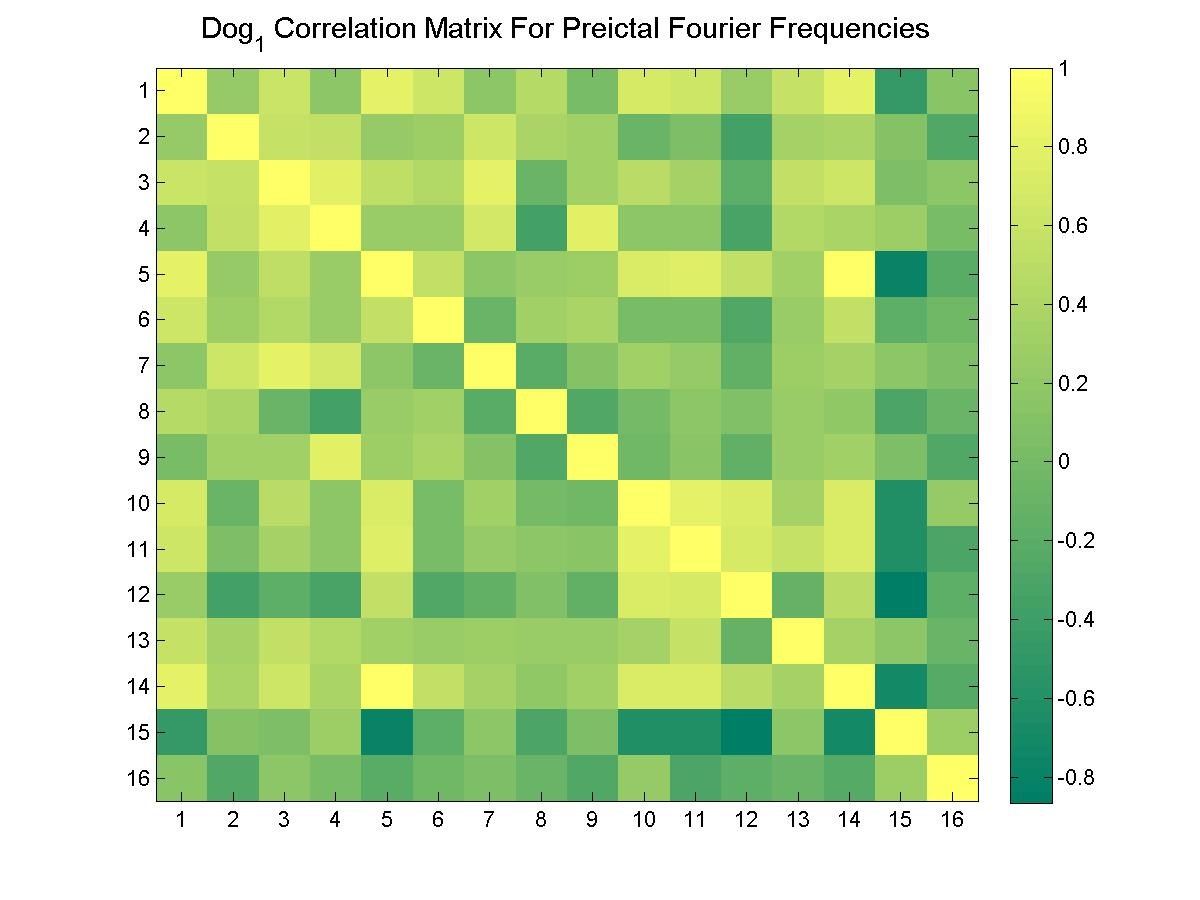
\includegraphics[width=0.4\linewidth]
{Dog1_PreictalFourierCorrelationPlot.jpg} }}
	\caption{Correlation heatmap among principal frequencies for different electrodes in Dog1 data}
	\label{d1freqcorr}
\end{figure}

Other bi-variate features mentioned in the paper, that we can study and use, are as follows:
\begin{enumerate}
\item Maximal cross-correlation between pairs of EEG channels
\item Nonlinear interdependence, i.e., the Euclidean distance, in reconstructed state-space, between trajectories described by two EEG channels \cite{arnhold}
\end{enumerate}

\subsection{Fourier spectra as features to logistic regression model}
As also mentioned in \ref{spec}, we can take the vector of amplitudes obtained on Fourier decomposition of each electrode's signal and use it as a feature vector to train a logistic regression model. This choice of model is supported by the claim in \cite{lecun}, wherein they mention the use of patient-specific machine learning-based classifiers (support vector machines, logistic regression or convolutional neural networks). 

As the size of such a feature vector can become very large (number of electrodes * number of frequencies), we plan to use a low band pass filter. This is meaningful because we can observe from the fourier spectra shown in \ref{spec} that the amplitudes past a certain frequency (around 100 Hz) are almost 0. We do not expect sinusoidal waves of high frequency to show up in neural activity anyway.

\subsection{Fourier SVM}
Since the data is approximately periodic, as can be observed from the EEG plots, we can apply a Fourier SVM for classification. Since our data is huge, we intend to sample out data-points from the given signals and then pass them to SVM learner.

\begin{thebibliography}{99}
\bibitem{lecun} Piotr Mirowski, Deepak Madhavan, Yann LeCun, Ruben Kuzniecky (2008) \textit{Classification of Patterns of EEG Synchronization for Seizure Prediction} IEEE Workshop on Machine Learning for Signal Processing.
\bibitem{arnhold} Klaus Lehnertz, Ralph G. Andrzejak, Jochen Arnhold, Thomas Kreuz (2001) \textit{Nonlinear EEG Analysis in Epilepsy: Its Possible Use for Interictal Focus Localization, Seizure Anticipation, and Prevention} Journal of Clinical Neurophysiology.
\bibitem{yunpark} Yun Park, Lan Luo, Keshab K. Parhi, and Theoden Netoff(2011) \textit{Seizure prediction with spectral power of EEG using cost-sensitive support vector machines}

\end{thebibliography}

\end{document}